\documentclass[main.tex]{subfiles}

\pagestyle{fancy}
\fancyhf{}
\fancyhead[LE]{\makebox[\pageoffset][l]{\bfseries\thepage}\bfseries\leftmark}
\fancyhead[RO]{\bfseries\rightmark\makebox[\pageoffset][r]{\bfseries\thepage}}

\begin{document}

\section*{Goal}
Today we will preform experiments to determine the density of several unknown objects and an unknown fluid by using the concepts we learned in Chapter~\ref{chap:Force} and Archimedes' Principle, which we will cover today. 

\section*{Equipment}
\begin{itemize}
\item
850 Universal Interface
\item
PASCO Capstone Software
\item
Force Sensor and lab pole for mounting the Force Sensor
\item
Two spheres: one less dense than water, one more dense than water. One 500 g mass. One irregular object of either aluminium or copper.
\item
Tall can for submerging objects in water.
\item
Vernier calipers
\item
String
\item
Container of a solution other than water at the lecture desk
\item
Triple-beam balance
\end{itemize}•

\section*{Theory}
In order to find the density of our various objects we will use \emph{Archimedes' Principle} which states that when a body is completely or partially immersed in a fluid, the fluid exerts and upward buoyant force on the body equal to the weight of the fluid displaced by the body. First we will need to know the weight of the object.
\begin{wrapfigure}{r}{0.5\textwidth}
\centering
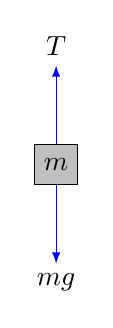
\begin{tikzpicture}[
	m/.style={rectangle,draw=black,fill=lightgray,minimum size=0.5cm,thin},
	force/.style={>=latex,draw=blue,fill=blue}
]
\node[m,left] (m) {$m$};
	\draw[force,->] (m.north) -- ++(0,1) node[above] {$T$};
	\draw[force,->] (m.south) -- ++(0,-1) node[below] {$mg$};
\end{tikzpicture}
\caption{Object in Air.}\label{fig:Air}
\end{wrapfigure}
~
\begin{wrapfigure}{R}{0.5\textwidth}
\centering
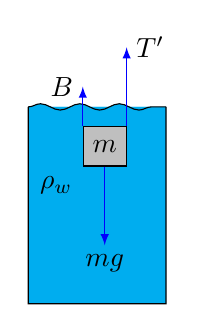
\begin{tikzpicture}[
	m/.style={rectangle,draw=black,fill=lightgray,minimum size=0.5cm,thin},
	force/.style={>=latex,draw=blue,fill=blue}
]
\coordinate (water-start) at (-1.25,0.5);
\coordinate (water-end) at (0.5,0.5);
\draw [fill=cyan] (water-start) -- ++(0,-2.5) -- ++(1.75,0) -- (water-end);
\draw[
    decoration={
        snake,
        amplitude =.4mm,
        segment length = 5mm
    },
    fill=cyan
] decorate {(water-start) -- (water-end)};

\node[m,left] (m) {$m$};
	\draw[force,->] (m.north east) -- ++(0,1) node[right] {$T'$};
	\draw[force,->] (m.north west) -- ++(0,0.5) node[left] {$B$};
	\draw[force,->] (m.south) -- ++(0,-1) node[below] {$mg$};

\node [xshift=3pt] (rho) at (-1,-.5) {$\rho_w$};
\end{tikzpicture}
\caption{Object in Water.}\label{fig:Water}
\end{wrapfigure}
From Figure~\ref{fig:Air} we can see that the net force on the object $m$ is,
\begin{equation}\label{eq:ForceAir}
\Sigma F = T-mg=0.
\end{equation}
Thus we can identify the true weight of the object as $T=mg.$ If we were to immerse our object in water and examine the forces acting on it now we can see from Figure~\ref{fig:Water} we can write,
\begin{equation}\label{eq:ForceWater}
\Sigma F = T'+B-mg=0,
\end{equation}
where $T'$ is the new scale reading and $B$ is called a \emph{buoyant force.} By solving Equation~\eqref{eq:ForceWater} and substituting in the true weight we have,
\begin{equation}\label{eq:B_tension}
B = T - T'.
\end{equation}
\FloatBarrier
But we know from Archimedes' Principle that we can write the buoyant force in terms of the weight of the displace fluid,
\begin{equation}\label{eq:B_weight}
B=m_w g,
\end{equation}
where $m_w$ is the mass of the displaced \emph{water}, not the mass of the object. We can define \emph{density} as the mass per unit volume or,
\begin{equation}\label{eq:density}
\rho=\frac{m}{V}.
\end{equation}
If we use this definition of density we can rewrite Equation~\eqref{eq:B_weight} as,
\begin{equation}\label{eq:B_density}
B = \rho_w V g.
\end{equation}
We can use the total volume $V$ of the object in Equation~\eqref{eq:B_density} because we are assuming that the object is completely submerged. However, given how we will be preforming the experiment, we want all our equations to be in terms of tensions that we can measure with the Force Sensor. To do this we need to look at Equation~\eqref{eq:density} again. If we take Equation~\eqref{eq:density} for the object and solve for $V$ we have,
\begin{align}
V&=\frac{m}{\rho_{obj}} \nonumber \\
&=\frac{T}{\rho_{obj}g}, \label{eq:VolumeT}
\end{align}
where in the second line we used the fact that the mass of the object, $m,$ is related to the tension of the string in air, $T.$ Substituting Equation~\eqref{eq:VolumeT} into Equation~\eqref{eq:B_density} and simplifying gives us,
\begin{equation}
B=\frac{\rho_w}{\rho_{obj}}T,
\end{equation}
which when equated to Equation~\eqref{eq:B_tension} and solved for $\rho_{obj}$ gives us our final expression,
\begin{equation} \label{eq:rho_obj}
\rho_{obj}=\frac{T}{T-T'}\rho_{w}.
\end{equation}

\begin{wrapfigure}[10]{r}{0.5\textwidth}
\centering
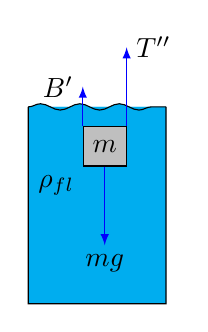
\begin{tikzpicture}[
	m/.style={rectangle,draw=black,fill=lightgray,minimum size=0.5cm,thin},
	force/.style={>=latex,draw=blue,fill=blue}
]
\coordinate (water-start) at (-1.25,0.5);
\coordinate (water-end) at (0.5,0.5);
\draw [fill=cyan] (water-start) -- ++(0,-2.5) -- ++(1.75,0) -- (water-end);
\draw[
    decoration={
        snake,
        amplitude =.4mm,
        segment length = 5mm
    },
    fill=cyan
] decorate {(water-start) -- (water-end)};

\node[m,left] (m) {$m$};
	\draw[force,->] (m.north east) -- ++(0,1) node[right] {$T''$};
	\draw[force,->] (m.north west) -- ++(0,0.5) node[left] {$B'$};
	\draw[force,->] (m.south) -- ++(0,-1) node[below] {$mg$};

\node [xshift=3pt] (rho) at (-1,-.5) {$\rho_{fl}$};
\end{tikzpicture}
\caption{Object in Unknown Fluid.}\label{fig:Fluid}
\end{wrapfigure}
To find the density of the unknown fluid we simply need to take one more step. By using our result from Equation~\eqref{eq:rho_obj} and a similar result that derives from Figure~\ref{fig:Fluid} we should be able to get the following equation for the density of the fluid,
\begin{equation} \label{eq:rho_fl}
\rho_{fl}=\frac{T-T''}{T-T'}\rho_{w}.
\end{equation}•

\section*{Procedure}

\begin{enumerate}
\item
Arrange the equipment so that the can rests on top of the lift and directly below the Force Sensor. Attach the object to the Force Sensor via a string.
\item
Fill the can about $^2\!/_3$--$^3\!/_4$ full of water.
\item
Measure the diameter of the two spheres with the vernier calipers.
\item
Open Capstone. Attach the Force Sensor to the 850UI and setup Capstone to use the Force Sensor in the appropriate port.
\item
Calibrate the Force Sensor as we did on page~\pageref{page:Calibration}, making sure to set the object's weight as a \emph{negative} value.
\item
Create a graph in Capstone to display the value of the Force Sensor. Click on the Statistics button 
\includegraphics{Statistics} to display the mean of the data.
\item \label{step:Archimedes_start}
Measure the masses of the two spheres using the scale.
\item
Zero the Force Sensor by pressing the tare button.
\item \label{step:T}
Determine the weight ($T$) of the the heavier sphere using the Force Sensor. The weight will be the mean value of our force data on the graph.
\item
Using the lift, raise the can up towards the Force Sensor until the sphere is completely submerged in the water.
\item \label{step:T'}
Determine the new tension ($T'$) in the string. Click on the Select Data Run button 
\includegraphics{Select_Data_Run} so that both $T$ and $T'$ values are shown on the graph.
\item \label{step:Archimedes_end}
Dry the sphere and remove the wet string.
\item \label{step:repeat}
Repeat steps~\ref{step:Archimedes_start}--\ref{step:Archimedes_end} for the remaining three objects. Print a graph for each object. n.b., to submerge the lighter sphere we need to tie it tightly to the heavier one. Use the two spheres together to measure the forces $T$ and $T'.$
\item \label{step:fluid}
Repeat steps~\ref{step:Archimedes_start}--\ref{step:Archimedes_end} for the heavier sphere, but using the unknown fluid at the lecture desk instead of water. \emph{Caution:} The fluid used may be poisonous, such as methyl alcohol or hydrochloric acid. Handle the container with care. Wash and dry the sphere after this step.
\end{enumerate}•

\section*{Analysis}
\begin{enumerate}
\item
Using the diameter measurements, determine the volume of the two spheres. Remember that the volume of a sphere is given by,
\[
V_{sphere}=\frac{4}{3}\pi r^3.
\]
\item \label{step:rho_volume}
Determine the densities of the two spheres using the mass and volume.
\item \label{step:rho_tension}
From the tensions measured in procedure steps~\ref{step:T},\ref{step:T'}, and \ref{step:repeat} calculate the densities of the four samples using Equation~\eqref{eq:rho_obj}. For the lighter sphere we will need to subtract the appropriate corresponding tensions of the heavier sphere from $T$ and $T'$ before calculating the density.
\item
Using Equation~\eqref{eq:rho_fl} and the measurements from procedure step~\ref{step:fluid} determine the density of the unknown fluid.
\item
Compare the two methods of calculating the density for the two spheres as determined in analysis steps~\ref{step:rho_volume} and \ref{step:rho_tension}. Using the mass/volume (step~\ref{step:rho_volume}) result as the standard, give a percent discrepancy for each sphere.
\item
Compare the density of the irregular object with either copper ($8960 \text{kg}/\text{m}^3$) or aluminium ($2700 \text{kg}/\text{m}^3$) as appropriate for the sample.
\item
Compare the density of the unknown fluid with those on the list displayed in the laboratory classroom. Identify the liquid and give a percent discrepancy.
\end{enumerate}•

\begin{samepage}
\hrulefill\\ \\
\emph{Chapter~\ref{chap:Archimedes}:} \textbf{Archimedes' Principle (Major Report)}
\begin{enumerate}
\item
\textbf{(5)} Title page (Experiment name, date, author, lab partner names)
\item
\textbf{(10)} Objective/Goal/Purpose --- Should have two parts: What is the overall physics principle or principles we are using and what are we actually determining in this lab. 
\item
\textbf{(25)} Theory --- Theory section included both complete sentences and equations. For this report, free body diagrams are required. Name the physics principles we use. Name and define any physical quantities that are used. Derive any equations that we use in our calculations from first principles. List, but do not derive the volume of a sphere formula. Be sure to include any error formulas we use (percent discrepancy).
\item
\textbf{(10)} Equipment --- Make a list of the equipment used and a sketch of the experimental setup. If it is not obvious identify what each part does in the experiment. e.g., what is the paper clip used for?
\item
\textbf{(10)} Procedure --- Give a brief description of each step of the experiment.
\item
\textbf{(25)} Data \& Data Analysis --- Present the data in a nicely organized table including units. Make sure the number of significant figures reflects the precision of the measurements. Present the results of the analysis in an organized way, clearly identifying what each number represents. Give a sample calculation for each new quantity that is presented.
\item
\textbf{(10)} Error Analysis --- Discuss at least three sources of experimental error. Human error is \emph{not} an acceptable source. Is the error large or small? Is it systematic or random? Give reasons for each. Also, discuss what could be done to reduce the errors in each case.
\item
\textbf{(5)} Conclusion --- What actual quantities were measured to within what error? (Percent discrepancy.) Were the underlying physical principles verified? (Were the errors small enough?)
\end{enumerate}•
\end{samepage}

\newpage
\section{Data Sheet}
\begin{doublespace}
Diameters of spheres:\\
$d_H=\rule[-1mm]{2.5cm}{.1pt}\pm\rule[-1mm]{1.5cm}{.1pt} \quad d_L=\rule[-1mm]{2.5cm}{.1pt}\pm\rule[-1mm]{1.5cm}{.1pt}$\\
Masses of spheres:\\
$m_H=\rule[-1mm]{2.5cm}{.1pt} \quad m_L=\rule[-1mm]{2.5cm}{.1pt}$\\[1cm]

\noindent
\begin{tabular}{|c|c|c|c|c|}
\hline
Object & Heavy sphere & Heavy \& Light spheres & 500 g mass & Irregular object\\
\hline
$T$ (N) &&&&\\
\hline
$T'$ (N) &&&&\\
\hline
$T''$ (N) &&\Vhrulefill&\Vhrulefill&\Vhrulefill\\
\hline
\end{tabular}
\end{doublespace}
\end{document}
